\section{Puntos Importantes}
A continuación presento algunos de los puntos más importantes que presentaron durante el reporte del IPCC: 


\subsection{\textcolor{red}{La importancia de medio grado}}
Este medio grado de medio grado es la diferencia que hay entre la vida y la muerte para muchas especies animales, así como la supervivencia de importantes ecosistemas marinos como lo es el coral, siendo este el hogar de muchas especies pequeñas que se encuentran al principio de la cadena alimenticia. Se estima que si la temperatura llega a los $2^\circ$C se perderán el 99\% de estos, mientras que si la temperatura solo alcanza los $1.5^\circ$C solo se perderían del 70 al 90\%. \textcolor{blue}{"Limitar el calentamiento global a $1.5^\circ$C en comparación con $2^\circ$C reduciría los impactos desafiantes sobre los ecosistemas, la salud humana y el bienestar, facilitando el logro de los Objetivos de Desarrollo Sostenible (ODS) de las Naciones Unidas}, dijo Priyardarshi Shukla, Co-presidente del Grupo de Trabajo III del IPCC.

\subsection{\textcolor{red}{Es posible, debemos movernos rápido}}
\textcolor{blue}{"Limitar el calentamiento a $1.5^\circ$C es posible dentro de las leyes de química y física, pero hacerlo requeriría cambios sin precedentes}, dijo Jim Skea, Co-presidente del Grupo de trabajo III del IPCC. Se recalca la necesidad de reducir las emisiones de $CO_2$ en al menos un 45\% para el 2030 con respecto a las de 2010 y continuar con los esfuerzos para alcanzar cero emisiones para 2050. Para lograr esto el informe nos exhorta a hacer grandes cambios en el uso de la tierra y la generación de energía para la industria, transportes y edificios en todas las ciudades del mundo. Es un desafío enorme el de mantenernos por debajo $2^\circ$C, ya que requiere que la infraestructura de combustibles fósiles se elimine gradualmente y que se elimine carbono a gran escala de la atmósfera, dice Glen Peters , Director de Investigación en el Centro de Investigación Climática Internacional de Noruega. \textcolor{blue}{"Mantenerse por debajo de 1.5 C simplemente requiere que la transformación sea más rápida y más profunda que para $2^\circ$C}, dijo Peters.

\subsection{\textcolor{red}{Soluciones Presentadas}}
En el reporte del IPCC se establecen varias soluciones para lograr la meta de $1.5^\circ$C, sin embargo, todas requieren  
esfuerzos sin precedentes para reducir la quema de combustibles fósiles en menos de 10 años y que estos lleguen a 0 en 30 años. Es decir, para medio siglo debemos lograr que ningún hogar, negocio o edificio debe calentarse a base de gas o petroleo, no más vehículos alimentados por Diesel o gasolina y aquellas industrias de producción pesada debe utilizar fuentes de energía limpia o bien, almacenar sus emociones de $CO_2$ permanentemente. Esto significara un gasto enorme de capital por parte de las empresas para apegarse al plan de reducción o un paro total de sus actividades lo que implicaría que estas cierren sus puertas como es el caso de centrales eléctricas y de gas.
\begin{figure}[H]
  \centering 
  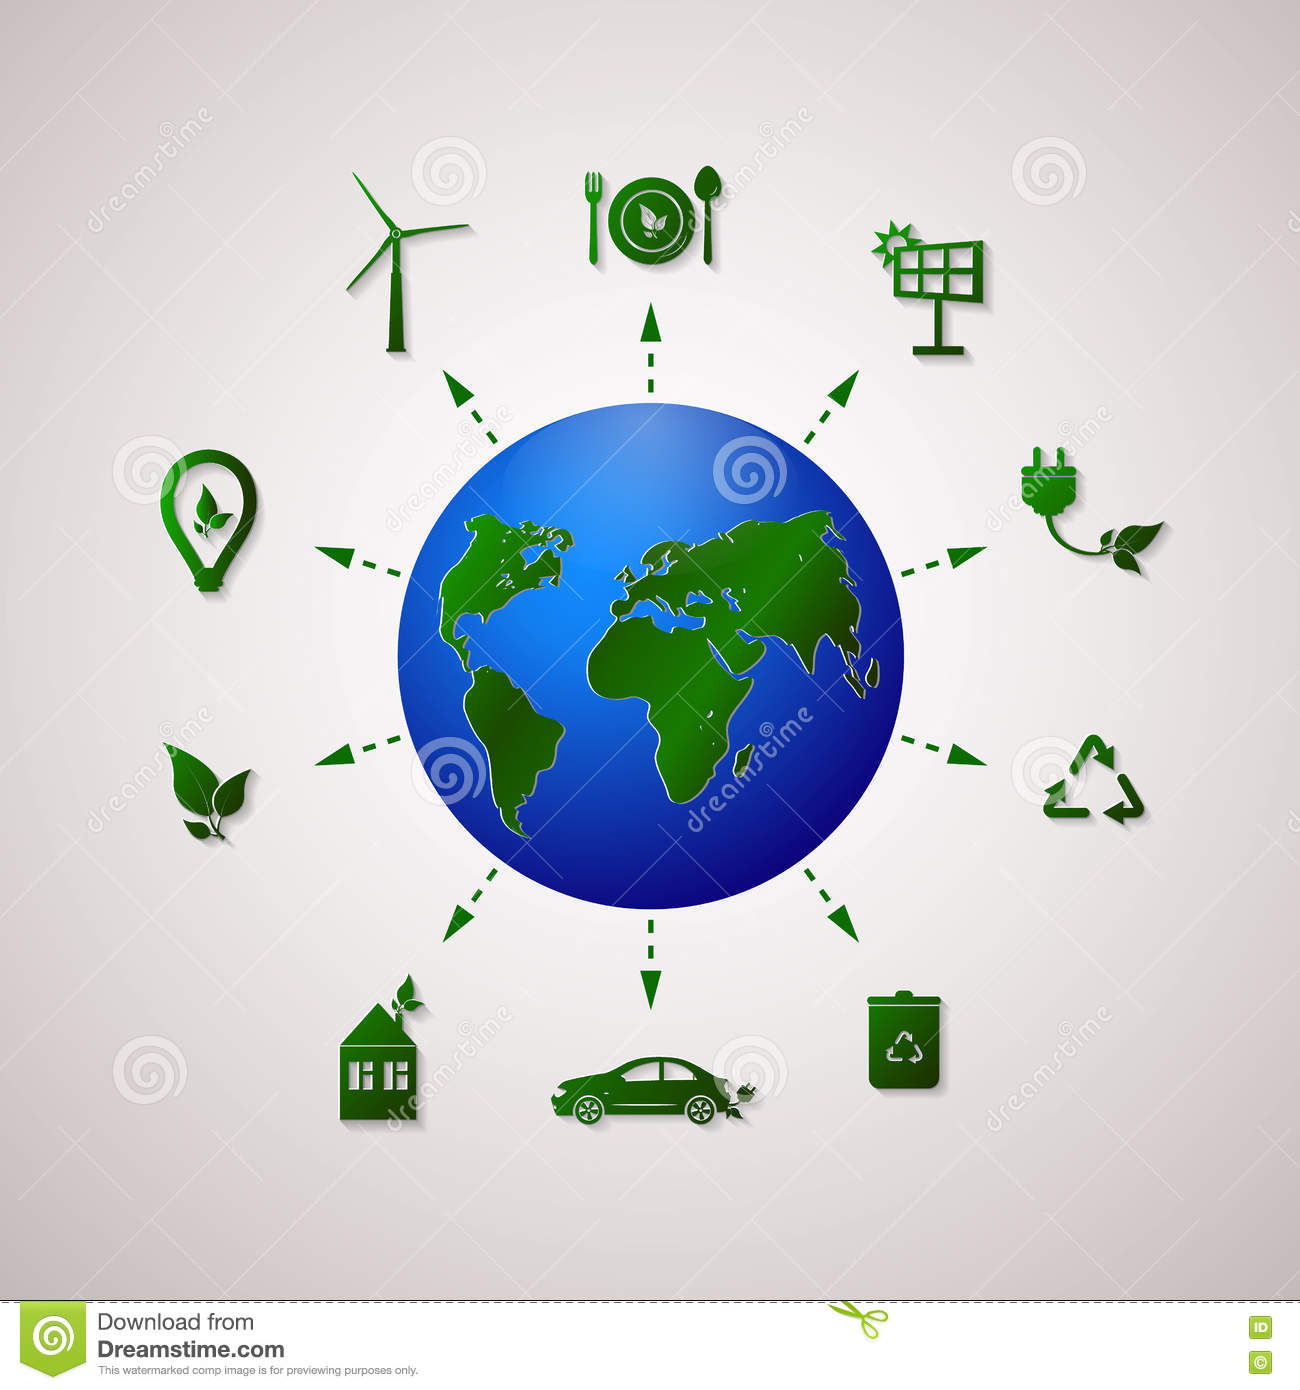
\includegraphics[width=0.15\textwidth]{figuras/planeta.jpg}
  \caption{Imagen de Dreamstime.com}
  \label{fig:revista_inatel}
\end{figure}

\subsection{\textcolor{red}{Reforestación y áreas verdes}}
En el reporte que se requiere de 1 a 7 millones de $Km^2$ de tierras convertidas en cultivos de bioenergía y hasta 10 millones de $Km^2$ más de bosques para el 2050. Para Deborah Lawrence , experta en bosques de la Universidad de Virginia, los bosques desempeñan un papel muy mucho mas importante en la reducción de las emisiones, pues según ella \textcolor{blue}{"Los bosques brindan un servicio súper importante para la humanidad al eliminar actualmente un 25\% del $CO_2$ de la atmósfera}. la reforestación representa un 18\% de las reducciones necesarias para el año 2030 dice Lawrence, países como Brasil, China, India, México, Australia, Estados Unidos, Rusia y la Unión Europea se están sumando a la reforestación. Proteger e incrementar los bosques tropicales es especialmente importante ya que enfrían el aire y son clave para crear precipitaciones regionales para el cultivo de alimentos.


